\documentclass{article}
\usepackage{neurips_2026}
\usepackage[utf8]{inputenc}
\usepackage[T1]{fontenc}
\usepackage{hyperref}
\usepackage{url}
\usepackage{booktabs}
\usepackage{amsfonts,amsmath,amssymb,amsthm}
\usepackage{nicefrac}
\usepackage{microtype}
\usepackage{xcolor}
\usepackage{graphicx}
\usepackage{enumitem}
\usepackage{caption}
\captionsetup{font=small,skip=3pt}
\newtheorem{proposition}{Proposition}
\providecommand{\textsc}[1]{#1}

\title{How Accurate Is Regression-Based Global Effect Estimation Under Network Interference? Leverage, Extrapolation and Misspecification}

\author{Anonymous Authors}

\begin{document}
\maketitle

\begin{abstract}
Regression-based estimators of the global average treatment effect (GATE) under network interference fit outcomes on a unit's treatment and neighbourhood exposure, then predict outcomes with everyone and with no one treated. How accurate can they be, and what determines their error? We decompose the error into a design-leverage term and an extrapolation-bias term and derive closed forms for the one-hop fraction regression: $\mathrm{RMSE}^2\approx B^2+\kappa L/n$, with $L=(1+d_H)/(p(1-p))$ under unit randomization ($d_H$ the harmonic-mean degree) and a cluster-design analogue, plus bias formulas for nonlinear exposure response (the regression recovers the response slope at $p$, not the secant), omitted multi-hop spillover ($\approx-\beta\lambda^2/(1-\lambda)$) and degree-related heterogeneity (a $1/d_i$-weighted estimand). In simulations on synthetic graphs and two Facebook graphs (Stanford3, ego-Facebook) with exactly known GATE, one fitted constant predicts the RMSE of 162 Bernoulli-design runs (median ratio $1.01$, $98\%$ within $10\%$) and the bias formulas match simulation to within about $0.01$--$0.02$ on a GATE of $2$. Biases do not shrink with $n$; cluster randomization helps in proportion to how well the graph clusters; richer regressions help only where the graph supplies units with extreme exposures; regression beats difference-in-means only when spillover exceeds $\approx\hat\kappa\sqrt{L/n}$; sandwich intervals cover well when the model is right (mean $0.95$) and fail when it is not ($0.57$). Outcomes are synthetic, and the closed forms are population-level and approximate for cluster designs.
\end{abstract}

\section{Introduction}
\label{sec:intro}

Online A/B tests on social networks and marketplaces violate the no-interference assumption: a unit's outcome depends on the treatments of its neighbours. The quantity a platform usually wants is the \emph{global average treatment effect} (GATE), $\tau=\frac1n\sum_i[Y_i(\mathbf 1)-Y_i(\mathbf 0)]$, the difference between mean outcomes if everybody and if nobody were treated. The usual difference in means (DiM) is biased for it. Inverse-probability (Horvitz--Thompson, H\'ajek) estimators of exposure-based contrasts~\citep{aronow2017estimating,ugander2013graph} are unbiased for the GATE under a correct exposure model, but need units whose whole neighbourhood is treated (or untreated); on dense graphs such units barely exist and variance explodes. \emph{Regression-based} estimators~\citep{chin2019regression,han2023model} sidestep this: fit $y_i$ on the unit's treatment and graph-derived exposure features from the experimental data, then predict outcomes under the all-treated and all-control assignments and average the difference. They use every unit and are cheap, but how accurate they can be, what determines their error, and when they fail is only partly understood.

\paragraph{This paper.} We study these questions with controlled simulations on synthetic graphs (Erd\H{o}s--R\'enyi, stochastic block model, Watts--Strogatz, Barab\'asi--Albert, random regular) and two public Facebook graphs (Stanford3, $n=11{,}586$; ego-Facebook, $n=4{,}039$), with synthetic outcomes so that the true $\tau$ is known exactly. The device is a decomposition (Sec.~\ref{sec:theory}) of the error into a \emph{design-leverage} term, set by how far the all-treated/all-control exposures lie from those the design generates, and a \emph{bias} term set by misspecification, with closed forms for the one-hop fraction-of-treated-neighbours regression. Findings:
\begin{enumerate}[leftmargin=*,itemsep=1pt,topsep=2pt]
\item \textbf{Sampling error is predictable from graph and design alone.} $\mathrm{RMSE}\approx\hat\kappa\sqrt{L/n}$ with leverage $L=(1+d_H)/(p(1-p))$ under unit randomization ($d_H$: harmonic-mean degree): error grows like $\sqrt{\text{degree}}$, shrinks like $n^{-1/2}$, and one fitted constant predicts 162 Bernoulli-design runs with median ratio $1.01$ ($98\%$ within $\pm10\%$). Cluster randomization lowers $L$ by an amount that depends on how well the graph clusters (RMSE $2.9\times$ lower on ego-Facebook, $1.9\times$ on Stanford3); the closed form is a rough guide there.
\item \textbf{Four bias mechanisms with closed-form predictions that match simulation:} extrapolation under nonlinear exposure response (the regression recovers the slope at $p$, not the secant; Prop.~\ref{prop:extrap}); omitted multi-hop spillover ($B\approx-\beta\lambda^2/(1-\lambda)$; Prop.~\ref{prop:mh}); effect heterogeneity (OLS targets a $1/d_i$-weighted average of unit effects; Prop.~\ref{prop:wt}; bias up to $100\%$ of the GATE on Stanford3); exposure mis-definition. None shrinks with $n$; predicted bias and leverage jointly match the RMSE of 360 Bernoulli world-settings (median ratio $1.005$).
\item \textbf{Design matters as much as the estimator.} Clustering cuts leverage and, where the graph clusters well, bias (multi-hop bias $-0.71\to-0.11$ on ego-Facebook, $-0.85\to-0.49$ on Stanford3, little on ER/SBM); the treated fraction and number of clusters trade bias for variance.
\item \textbf{Rules and negative results.} Regression beats DiM only if spillover exceeds $\approx\hat\kappa\sqrt{L/n}$ ($\ge0.8\beta$ for $n{=}10^3$, $d{=}128$); H\'ajek estimators are undefined on dense random graphs ($d\ge32$) under unit randomization; richer regressions reduce bias only where the graph supplies extreme exposures (a cubic fixes Stanford3/ego-Facebook for $15$--$45\%$ extra RMSE but has RMSE $\approx2$ on near-regular graphs); sandwich intervals cover well when the model is right (mean $0.95$) and fail when it is not (mean $0.57$), the failure being explained by the bias.
\end{enumerate}
\section{Related work}
\label{sec:related}
\textbf{Designs and exposure-based estimation.} \citet{aronow2017estimating} give randomization-based inverse-probability estimators for general exposure mappings; graph cluster randomization~\citep{ugander2013graph}, its randomized variant~\citep{ugander2023randomized} and rate-optimal cluster designs~\citep{leung2022rate} reduce the variance of such estimators; \citet{eckles2017design} study interference bias and neighbourhood-aware analysis; \citet{karrer2021network} describe a deployed system; \citet{chen2023optimized} optimize assignment covariances for HT estimators. \textbf{Outcome models.} \citet{cortez2022staggered,cortez2023exploiting} and \citet{eichhorn2024low} obtain total-effect estimators under low-order interaction models (the last with clustered designs); \citet{yu2022estimating} work without the network. \citet{chin2019regression} proposes the regression-adjustment estimator studied here; \citet{han2023model} select graph- and treatment-based covariates with block bootstrap. \citet{savje2021average} and \citet{li2022random} give asymptotics under limited interference and random graphs. \textbf{This work} asks a diagnostic question about the regression estimator family: what determines its error, and which factor dominates when. Our contributions are closed-form leverage and bias predictors validated against simulation on real graph topologies, a head-to-head with difference-in-means and H\'ajek baselines, and an audit of interval coverage. We propose no new estimator; the weighted and stratified fits in Sec.~\ref{sec:results} are diagnostics-motivated fixes whose merits we only evaluate.

\section{Setting, estimators and metrics}
\label{sec:setting}
\textbf{Setting.} A connected undirected graph with adjacency $A$ on $n$ units, degrees $d_i\ge1$, $W=D^{-1}A$. Assignment $z\in\{0,1\}^n$ is drawn either by \emph{Bernoulli}$(p)$ (independent units) or by \emph{cluster randomization}: units are partitioned into clusters (Louvain communities~\citep{blondel2008fast}, resolution tuned to a target number $K$ of clusters) and clusters are independently treated with probability $p$ (redrawing the rare assignments in which one arm is empty). Potential outcomes $Y_i(z)$ are fixed given a ``world'' (graph plus unit-level parameters); the only randomness within a world is $z$. Exposure features are $s_i=(Wz)_i$ (fraction of treated neighbours), $c_i=(Az)_i$ (count), $s^{(2)}_i=(W^2z)_i$ (two-step fraction).

\textbf{Regression estimators.} $\hat\tau=\frac1n\sum_i[\hat f(x_i(\mathbf 1))-\hat f(x_i(\mathbf 0))]$ where $x_i(z)$ are the features and $\hat f$ is fitted on the observed data. Linear models: $(1,z,s)$ [\textsc{ols-s}, the default, Chin-type]; $(1,z,c)$ [\textsc{ols-cnt}]; $+zs$ [\textsc{int}]; $+s^2$ [\textsc{quad}]; $+s^2,s^3$ [\textsc{cub}]; $+s^{(2)}$ [\textsc{ols-s2}]; $+s\cdot\ell_i,\ \ell_i$ (standardized log degree) [\textsc{s-deg}]; weighted least squares with weights $\propto1/\mathrm{Var}(s_i)$ [\textsc{wls-s}]; separate \textsc{ols-s} fits in five degree strata, averaged with stratum sizes [\textsc{strat-s}]; gradient boosting (scikit-learn HistGradientBoosting) on $(z,s,s^{(2)},\ell)$ [\textsc{gbm}]. \textbf{Baselines:} DiM; H\'ajek estimator with exposure ``unit and all neighbours treated'' / ``none treated'' with exactly computed design probabilities (undefined when no unit qualifies in an arm).

\textbf{Metrics.} For each setting we report, over $R=300$ assignments in each of $6$ independent worlds, the \emph{bias} $\mathbb E\hat\tau-\tau$, \emph{SD}, and \emph{RMSE}$=\sqrt{\mathbb E(\hat\tau-\tau)^2}$; RMSE is our headline metric because it combines bias and variance, which have different drivers; we show both. Tables and figures give means across worlds with min--max across the 6 worlds as error bars (Monte-Carlo standard errors of each world's RMSE are $\le0.04\times$RMSE with $R=300$ and are smaller than the across-world spread). For inference we report empirical coverage of nominal 95\% intervals $\hat\tau\pm1.96\,\widehat{\mathrm{se}}$.

\section{What determines the error: a decomposition and closed-form predictors}
\label{sec:theory}

Throughout, the randomness is the assignment $z$ only (design-based); potential outcomes are fixed. Let $\phi_i(z)\in\mathbb R^k$ be the feature map, $\hat\Sigma=\frac1n\sum_i\phi_i\phi_i^\top$ and $\hat\beta=\hat\Sigma^{-1}\frac1n\sum_i\phi_iy_i$. The estimator is $\hat\tau=\bar d^\top\hat\beta$ with $\bar d=\frac1n\sum_i[\phi_i(\mathbf 1)-\phi_i(\mathbf 0)]$ (for $\phi=(1,z,s)$: $\bar d=(0,1,1)$). Let $\Sigma=\mathbb E\hat\Sigma$, $\beta^\star=\Sigma^{-1}\frac1n\sum_i\mathbb E[\phi_iy_i]$ be the population least-squares coefficient under the design, $\varepsilon_i=y_i-\phi_i^\top\beta^\star$ and $\hat g=\frac1n\sum_i\phi_i\varepsilon_i$ (so $\mathbb E\hat g=0$).

\begin{proposition}[Decomposition]\label{prop:decomp}
Exactly, $\hat\tau-\tau=B+\bar d^\top\hat\Sigma^{-1}\hat g$ with the \emph{extrapolation bias} $B=\bar d^\top\beta^\star-\tau$, which does not depend on $n$ through any sampling effect. To first order ($\hat\Sigma\to\Sigma$) the second term has mean zero and variance at most $\kappa L/n$, where $L=\bar d^\top\Sigma^{-1}\bar d$ is the \emph{design leverage} of the all-treated-vs-all-control contrast and $\kappa=\lambda_{\max}\big(\Sigma^{-1/2}\,n\mathrm{Cov}(\hat g)\,\Sigma^{-1/2}\big)$ is the effective residual scale ($\kappa\approx\sigma^2$ for homoskedastic independent residuals). Hence $\mathrm{RMSE}^2\approx B^2+\kappa L/n$.
\end{proposition}

$L$ depends on the graph, design and feature map but not on the outcomes: it is the price of extrapolating from the exposures the design generates to the corners ``everyone treated'' and ``no one treated''. For $\phi=(1,z,s)$ (Chin-type estimator) it has a closed form.

\begin{proposition}[Leverage of the one-hop fraction model]\label{prop:lev}
Let $v=p(1-p)$, $w_{ic}=m_{ic}/d_i$ where $m_{ic}$ is the number of neighbours of $i$ in cluster $c$, $\rho=\frac1n\sum_i w_{i,c(i)}$ and $q=\frac1n\sum_i\sum_c w_{ic}^2$. Under independent cluster-level Bernoulli$(p)$ assignment (unit-level Bernoulli is the case of singleton clusters, $\rho=0$, $q=1/d_H$ with $d_H=(\frac1n\sum_i 1/d_i)^{-1}$ the harmonic-mean degree),
\[
L=\frac{1}{v}\Big[1+\frac{(1-\rho)^2}{q-\rho^2}\Big],\qquad\text{in particular}\qquad L_{\rm Bern}=\frac{1+d_H}{p(1-p)} .
\]
\end{proposition}

The interference penalty over the no-interference variance $1/v$ is $(1-\rho)^2/(q-\rho^2)$: $d_H$ for unit randomization, $\to0$ when all neighbours share the unit's cluster ($\rho\to1$; $z$ and $s$ collinear, as precise as DiM). So $\mathrm{RMSE}\propto\sqrt{(1+d_H)/(vn)}$ under unit randomization.

\begin{proposition}[Extrapolation bias under a nonlinear exposure response]\label{prop:extrap}
Let $Y_i(z)=a_i+\beta_iz_i+\gamma\,g(s_i)$ with $g(0)=0,\ g(1)=1$, and Bernoulli$(p)$ assignment (heterogeneous $\gamma_i$ with mean $\gamma$, independent of degree, give approximately the same $B$). For $\phi=(1,z,s)$,
\[
B=\gamma\,(\kappa_p-1),\qquad \kappa_p=\frac{\sum_i\mathrm{Cov}(g(s_i),s_i)}{\sum_i\mathrm{Var}(s_i)},\quad s_i\sim\mathrm{Bin}(d_i,p)/d_i ,
\]
and $\kappa_p\to g'(p)$ when all degrees grow, so that $B\to\gamma\,(g'(p)-1)$: \emph{the regression recovers the slope of the response at $p$, not the secant slope between $0$ and $1$.}
\end{proposition}

For $g(s)=s^k$ at $p=\tfrac12$, $g'(p)=k2^{1-k}$: $B=0$ for $k=2$ (tangent at $\frac12$ equals secant), $-\gamma/2$ for $k=4$, $\approx-0.29\gamma$ for $k=\frac12$; steep thresholds centred at $p$ give large positive bias. $B$ is not reduced by more data, nor (Sec.~\ref{sec:results}) by more flexible regressions when, under unit randomization with large degree, essentially no unit has exposure near $0$ or $1$.

\begin{proposition}[Heterogeneous effects: the estimand is variance-weighted]\label{prop:wt}
Let $Y_i(z)=a_i+\beta_iz_i+\gamma_is_i$ and Bernoulli assignment. For $\phi=(1,z,s)$, $\beta^\star$ yields
$\;\bar d^\top\beta^\star=\bar\beta+\sum_i\pi_i\gamma_i,\ \pi_i=d_i^{-1}/\sum_jd_j^{-1}$, whereas $\tau=\bar\beta+\bar\gamma$ (uniform weights). The bias is $B=\sum_i(\pi_i-\frac1n)\gamma_i$.
\end{proposition}

OLS weights unit effects by the variance $\propto1/d_i$ of the unit's exposure, so low-degree units dominate; if susceptibility correlates with degree the bias can be of the order of the effect itself, whatever $n$.

\begin{proposition}[Omitted multi-hop spillover]\label{prop:mh}
Let $Y(z)=(I-\lambda W)^{-1}(a+\beta z)$, $W=D^{-1}A$, $|\lambda|<1$, with Bernoulli assignment and $\phi=(1,z,s)$. Define $r_k=\frac1n\mathrm{tr}\,W^k$, $u_k=\frac1n\sum_{ij}(W^k)_{ij}W_{ij}$, $q=u_1$ and $\psi_k=r_k+u_k/q$. Then
\[ B=-\beta\sum_{k\ge2}\lambda^k(1-\psi_k)\;\approx\;-\beta\,\frac{\lambda^2}{1-\lambda}\quad(\psi_k\approx0).\]
\end{proposition}

$\psi_k$ is the share of $k$-step influence aliased with the included one-hop terms (return and closure probabilities); on tree-like graphs the regression misses all indirect effect beyond one hop. Under cluster randomization distant exposures correlate with $s$ and are partly absorbed (Sec.~\ref{sec:results}); we give no closed form for that case.

Proofs (Appendix~\ref{app:proofs}) are design-expectation statements; finite-$n$ and finite-cluster effects are quantified empirically.

\section{Experimental protocol}
\label{sec:protocol}

\textbf{Graphs.} Synthetic ($n=4000$ unless stated): Erd\H{o}s--R\'enyi (ER) and random regular with mean degree $d\in\{4,\dots,256\}$; stochastic block model (SBM, 40 equal blocks, $p_{\rm in}/p_{\rm out}=30$); Watts--Strogatz (WS, rewiring $0.05$; strong local clustering); Barab\'asi--Albert (BA, $m\in\{3,\dots,24\}$; heavy-tailed degrees). Real: Stanford3 (Facebook100~\citep{traud2012social}; Network Repository~\citep{rossi2015network}; $n=11{,}586$, $568{,}309$ edges, mean/median/max degree $98/73/1172$, mean local clustering $0.24$) and ego-Facebook (SNAP~\citep{mcauley2012learning}; $n=4{,}039$, $88{,}234$ edges, mean/median/max degree $44/25/1045$, clustering $0.61$). Both are connected. Data versions and checksums are in Appendix~\ref{app:repro}. Clusterability differs sharply: the Louvain partition into $\approx30$ clusters cuts $18\%$ of ego-Facebook's edges but $58\%$ of Stanford3's.

\textbf{Potential outcomes.} Unit-level draws are made once per world: baseline $a_i\sim N(0,1)$, direct effect $\beta_i=1+0.5\xi_i$, spillover coefficient $\gamma_i=\gamma(1+0.5\zeta_i)$, $\xi,\zeta\sim N(0,1)$ (so $\bar\beta\approx1$, $\bar\gamma\approx\gamma$, default $\gamma=1$). There is no extra observation noise; baselines and effect heterogeneity act as design-based noise. Mechanisms:
\textbf{(i)~one-hop fraction}, $Y_i=a_i+\beta_iz_i+\gamma_ig(s_i)$ with $g(s)=s^k$ (linear $k=1$; concave $k\in\{\frac14,\frac12\}$; convex $k\in\{2,4\}$) or a threshold response $g(s)\propto\sigma((s-\frac12)/0.08)$ rescaled to $g(0)=0,g(1)=1$ so that $\tau\approx\bar\beta+\bar\gamma$ for every shape; \textbf{(ii)~multi-hop} (linear-in-means equilibrium) $Y=(I-\lambda W)^{-1}(a+\beta z)$, $\lambda\in[0,0.8]$, $\tau=\bar\beta/(1-\lambda)$ in expectation; \textbf{(iii)~count}: $Y_i=a_i+\beta_iz_i+\gamma_ic_i/\bar d$; \textbf{(iv)~degree-heterogeneous} spillover: (i) with $\gamma_i\propto e^{\mp0.7\ell_i}$ ($\ell_i$ standardized log degree; ``inv'': low-degree units more susceptible; ``pos'': high-degree units), normalized to mean $\gamma$. The true $\tau$ is computed exactly from $Y(\mathbf1)-Y(\mathbf0)$.

\textbf{Experiments and worlds.} Seven experiments (E1--E7; scripts in Appendix~\ref{app:repro}) vary degree, $n$ and noise (E1); response shape (E2); neighbourhood, heterogeneity and exposure definition (E3); spillover strength (E4); treated fraction and number of clusters (E5); inference (E6); a mis-measured graph (E7). Each setting uses $6$ independent \emph{worlds} (a fresh synthetic graph and unit parameters, or fresh unit parameters on the fixed real graph) with $R=300$ assignments each ($400$ in E6, $40$ for \textsc{gbm}). Hypotheses H1--H6 (error $\propto$ leverage; persistent extrapolation bias; multi-hop omission bias; heterogeneity bias; clustering helps iff the graph clusters; regression beats DiM only above a spillover threshold) were fixed before the final runs. A three-world pilot of E1/E3 set the run scale and exposed a crash (assignments with an empty arm under few clusters), fixed in the released code; \textsc{wls-s} and \textsc{strat-s} were added after the pilot heterogeneity results and are labelled as such.

\section{Results}
\label{sec:results}

\subsection{Sampling error is set by design leverage (H1)}
With a correctly specified linear one-hop response, the RMSE of \textsc{ols-s} grows with mean degree with log-log slope $0.52$ in $\log(1+d)$ (ER) and falls with $n$ with slope $-0.50$ (Fig.~\ref{fig:var}a--b), as Prop.~\ref{prop:lev} implies. DiM does not improve with $n$ (its error is bias); H\'ajek is defined in more than half of the draws only for $n\ge8000$ at $d=16$ and has RMSE $1.3$--$1.4$ there. With one constant $\hat\kappa=1.09$ fitted on the 72 ER/Bernoulli runs, $\hat\kappa\sqrt{L/n}$ matches the observed RMSE of all 162 Bernoulli-design runs with median ratio $1.01$ and range $[0.85,1.13]$ ($98\%$ within $\pm10\%$; Fig.~\ref{fig:var}c), including the 90 non-ER runs (SBM, WS, BA, Stanford3, ego-Facebook) never used for fitting; simulated leverage equals the formula within $7\%$ for Bernoulli designs (App.~\ref{app:extra}).

\textbf{Cluster randomization lowers leverage; the closed form is rougher there.} With $\approx30$--$40$ clusters RMSE falls from $0.22$ to $0.04$ ($5\times$) on WS ($d{=}40$), from $0.120$ to $0.042$ ($2.9\times$; leverage $48.9\to5.6$) on ego-Facebook and from $0.071$ to $0.037$ ($1.9\times$; $47.1\to14.6$) on Stanford3, but only $1.2$--$1.6\times$ on SBM and $1.0$--$1.3\times$ on BA, whose clusterings cut $57\%$--$87\%$ of the edges. For the 126 cluster-design runs the formula underpredicts RMSE in $73\%$ (median ratio $1.10$, IQR $[1.00,1.29]$, range $[0.69,3.74]$); extremes occur with $\le10$ clusters, where one draw's sample covariance of $(z,s)$ differs from its expectation. Rank correlation between $\sqrt{L/n}$ and RMSE over all 288 runs is $0.96$.

\begin{figure}[t]
\centering
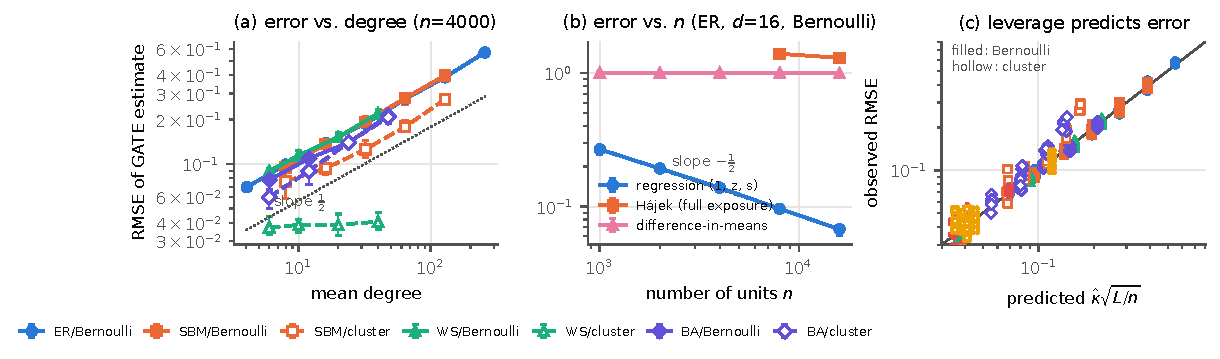
\includegraphics[width=\linewidth]{figs/fig_variance.pdf}
\caption{Variance side (E1). (a) RMSE of \textsc{ols-s} vs mean degree for five graph families under Bernoulli (solid) and cluster randomization (dashed, $K{=}40$ target clusters); dotted: slope $\frac12$. (b) RMSE vs $n$ on ER graphs with $d{=}16$: regression, H\'ajek (shown only where defined in $>50\%$ of assignments) and DiM. (c) Observed RMSE vs $\hat\kappa\sqrt{L/n}$ (closed-form leverage; one global $\hat\kappa$ fitted on ER/Bernoulli runs) for 288 runs including Stanford3 and ego-Facebook. Markers: mean over 6 worlds; bars: min--max over worlds (panels a--b); panel c shows each setting-world pair mean.}
\label{fig:var}
\end{figure}

\subsection{Extrapolation bias under nonlinear response does not vanish with $n$ (H2)}
Prop.~\ref{prop:extrap} gives the bias of the linear one-hop regression for any response shape from exact binomial moments. Over 63 (graph, shape, degree, $n$) Bernoulli settings the simulated bias differs from it by at most $0.012$ (median $0.003$) on a GATE of $\approx2$ (Fig.~\ref{fig:ext}a). It depends on the tangent slope at $p$: on ER ($d{=}30$) it is $\approx0$ for $k=2$, $-0.45$ for $k=4$, $-0.28$ for $k=\frac12$ and $+1.47$ for the threshold response (Appendix Table~\ref{tab:extrap}); it grows with degree as exposures concentrate near $p$ (Fig.~\ref{fig:ext}b) and is unchanged from $n=10^3$ to $1.6\times10^4$ (c). Combining the closed-form bias and leverage, $\sqrt{B^2+\hat\kappa^2L/n}$ matches the observed RMSE with median ratio $1.005$ (IQR $[0.99,1.03]$; $89\%$ within $\pm10\%$) over 360 world-settings (d).

\textbf{Flexible regressions help only where the graph provides extreme exposures.} Under Bernoulli($\frac12$) the share of units with $s\le0.1$ or $s\ge0.9$ is $0.0\%$ on ER/regular graphs ($d{=}30$), $0.5\%$ on BA, $6.5\%$ on Stanford3 and $4.3\%$ on ego-Facebook (and $79\%$ on ego-Facebook under cluster randomization). Where such units exist, a cubic in $s$ removes nearly all bias for every shape (Stanford3: $|$bias$|\le0.03$, RMSE $0.08$--$0.09$ vs $0.07$ for the linear model under a linear response; ego-Facebook: $|$bias$|\le0.07$, RMSE $0.17$--$0.18$ vs $0.12$), costing $15$--$45\%$ RMSE when the linear model was right. On ER the cubic has RMSE $1.9$--$3.1$ for all shapes and the quadratic leaves the bias unchanged (threshold: $1.47\to1.47$). Gradient boosting on $(z,s,s^{(2)},\ell)$ cannot extrapolate: even for a \emph{linear} response it is biased towards DiM ($-0.52$ on ER, $-0.24$ on Stanford3, $-0.13$ on ego-Facebook), but it has the lowest RMSE when the response is steep and the linear model badly wrong (threshold, Bernoulli: $0.52$ vs $1.47$ on ER, $0.26$ vs $0.38$ on Stanford3, $0.41$ vs $0.61$ on ego-Facebook) and is much worse when the linear model is adequate ($0.74$ vs $0.17$ on ER; 3 worlds, 40 assignments). Cluster randomization shrinks the linear model's bias where clusters are good (ego-Facebook $k{=}4$: $-0.22\to-0.03$; threshold $0.60\to0.05$) and little elsewhere (ER $k{=}4$: $-0.45\to-0.36$; Stanford3: $-0.13\to-0.12$).

\begin{figure}[t]
\centering
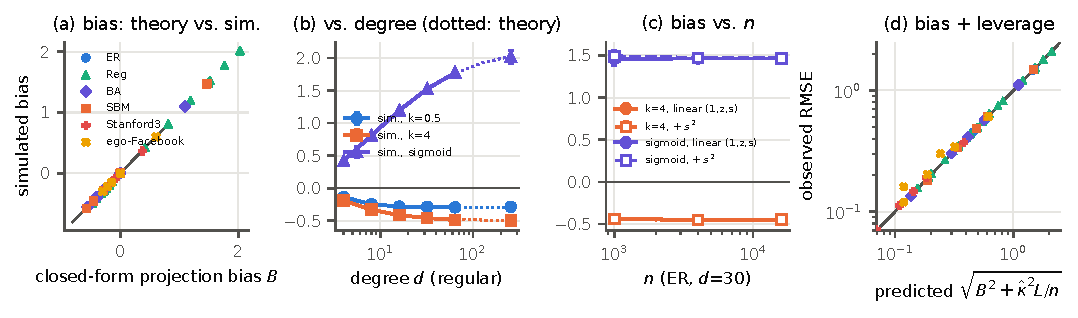
\includegraphics[width=\linewidth]{figs/fig_extrap.pdf}
\caption{Extrapolation bias (E2). (a) Simulated bias of \textsc{ols-s} vs the closed-form bias of Prop.~\ref{prop:extrap}, 63 Bernoulli settings (mean over 6 worlds). (b) Bias vs degree on random regular graphs ($n{=}4000$): simulation (solid; bars min--max) and theory (dotted). (c) Bias vs $n$, $k{=}4$ and threshold response, linear and $+s^2$ regressions. (d) Observed RMSE vs $\sqrt{B^2+\hat\kappa^2L/n}$ (closed-form $B$ and $L$, $\hat\kappa$ from E1).}
\label{fig:ext}
\end{figure}


\subsection{Misspecified neighbourhoods, heterogeneity and exposure definition (H3, H4)}
\textbf{Omitted multi-hop spillover.} Under the linear-in-means equilibrium the one-hop regression misses everything beyond one hop, and its bias follows Prop.~\ref{prop:mh} (Fig.~\ref{fig:mh}a; Appendix Table~\ref{tab:mh}): on ER ($d{=}30$) at $\lambda=0.6$ the simulated bias is $-0.872\pm0.007$ (s.e.\ over worlds) against $-0.867$ (exact walk-statistics formula) and $-0.900$ (tree-like approximation), a $35\%$ relative error of a GATE of $2.49$ independent of $n$; at $\lambda=0.8$ it is $63\%$. On triangle-rich ego-Facebook the tree-like formula fails ($-0.900$ vs simulated $-0.710$) but the exact one, using the graph's return/closure statistics $\psi_k$, does not ($-0.696$); on Stanford3 both agree ($-0.850$ exact vs $-0.846$). Adding the two-step exposure $s^{(2)}$ reduces the bias (ER, $\lambda{=}0.6$: $-0.87\to-0.55$; the rest comes from hops $\ge3$) but multiplies the SD by $5.4$ (ER), $4.0$ (Stanford3), $2.3$ (ego-Facebook) under Bernoulli ($\lambda{=}0.4$; leverage $3560$ vs $121$ on ER), so its RMSE is higher than the one-hop model's in 6 of 7 graph/design combinations at $\lambda=0.4$ and lower in 4 of 7 at $\lambda=0.6$ (all on real graphs). \textbf{Cluster randomization absorbs part of the omitted effect:} at $\lambda=0.6$ the bias falls from $-0.71$ to $-0.11$ on ego-Facebook, $-0.85$ to $-0.49$ on Stanford3, $-0.86$ to $-0.67$ on SBM, and grows again as clusters get finer (Fig.~\ref{fig:des}f).

\begin{figure}[t]
\centering
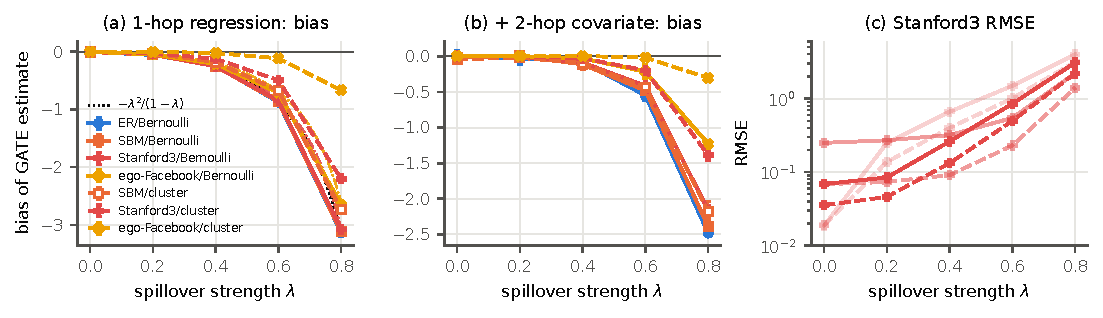
\includegraphics[width=\linewidth]{figs/fig_multihop.pdf}
\caption{Multi-hop interference (E3). (a) Bias of the one-hop regression vs $\lambda$ under Bernoulli (solid) and cluster designs (dashed) on four graphs; dotted black: tree-like prediction $-\lambda^2/(1-\lambda)$; dash-dotted: exact formula of Prop.~\ref{prop:mh} for ego-Facebook (yellow) and Stanford3 (red). (b) Bias after adding the two-step exposure. (c) RMSE on Stanford3: one-hop regression (dark), two-step regression (mid), DiM (light); solid Bernoulli, dashed cluster. Mean over 6 worlds, bars min--max.}
\label{fig:mh}
\end{figure}


\textbf{Heterogeneous susceptibility.} If $\gamma_i$ depends on degree, \textsc{ols-s} converges to a $1/d_i$-weighted average of unit effects (Prop.~\ref{prop:wt}; Table~\ref{tab:het}). On Stanford3 with ``inv'' heterogeneity (GATE $2.0$) the bias is $+2.04$ -- the estimate is twice the truth -- as predicted ($+2.03$, evaluated on the actual world parameters; per-world predictions and simulations agree within $0.02$); ``pos'': $-0.71$ ($-0.71$); ego-Facebook $+1.41$ ($+1.41$) and $-0.60$ ($-0.59$); BA graphs, with less degree spread, $+0.17$ and $-0.40$. Without degree-related heterogeneity it is unbiased ($|$bias$|\le0.01$). Adding the neighbour count or $s\times$log-degree reduces but does not remove the bias ($+1.55$, $-0.53$ on Stanford3 ``inv''). Variance-weighted fitting (\textsc{wls-s}) removes it ($+0.02$) but with RMSE $0.19$--$0.64$ (vs $0.07$--$0.12$ for \textsc{ols-s} in the homogeneous case); degree stratification (\textsc{strat-s}) gives bias $+0.20$, RMSE $0.27$ (vs $2.04$) and is almost free under cluster randomization (RMSE $0.04$--$0.05$). Both were devised after the pilot results.

\textbf{Exposure definition.} If spillover follows the neighbour \emph{count} (scaled by mean degree) but the model uses the \emph{fraction}, \textsc{ols-s} is biased by $-0.90$ (Stanford3) and $-0.75$ (ego-Facebook); the converse mismatch gives $-0.98$ and $-0.97$ (RMSE $0.98$). Including both $s$ and $c$ fixes both directions (RMSE $0.07$/$0.12$ under the fraction and $0.07$/$0.13$ under the count mechanism, vs $0.03$/$0.06$ for the correct count model), provided the true exposure is nested in the model.

\begin{table}[t]\centering\footnotesize\setlength{\tabcolsep}{3pt}
\caption{Degree-heterogeneous spillover (E3): bias (RMSE); true GATE $\approx2$. ``inv'': low-degree units are more susceptible, ``pos'': high-degree units. $B$: bias predicted by Prop.~\ref{prop:wt} for \textsc{ols-s}. $+c$: model with $s$ and the neighbour count; \textsc{s-deg}: $s$ and $s\times$log-degree; \textsc{wls-s}: weights $1/\mathrm{Var}(s_i)$; \textsc{strat-s}: separate fits in 5 degree strata (the last two designed after the pilot, see text). Mean over 6 worlds.}
\label{tab:het}
\begin{tabular}{lllcccccc}\toprule
graph & $\gamma_i$ het. & design & $B$ (Prop.~\ref{prop:wt}) & \textsc{ols-s} & $+c$ & \textsc{s-deg} & \textsc{wls-s} & \textsc{strat-s} \\
\midrule
Stanford3 & none & Bern. & -0.00 & -0.01 (0.07) & +0.00 (0.07) & +0.01 (0.16) & +0.00 (0.19) & +0.00 (0.19) \\
 &  & cluster & -- & -0.00 (0.04) & +0.00 (0.04) & -0.00 (0.04) & -0.00 (0.05) & +0.00 (0.04) \\
 & inv & Bern. & +2.03 & +2.04 (2.04) & +1.55 (1.56) & -0.53 (0.56) & +0.02 (0.21) & +0.20 (0.27) \\
 &  & cluster & -- & +0.65 (0.70) & +0.35 (0.37) & -0.08 (0.13) & +0.21 (0.30) & +0.08 (0.09) \\
 & pos & Bern. & -0.71 & -0.71 (0.71) & -0.25 (0.26) & -0.18 (0.24) & +0.00 (0.26) & -0.04 (0.21) \\
 &  & cluster & -- & -0.34 (0.38) & -0.07 (0.09) & -0.05 (0.07) & -0.14 (0.24) & -0.02 (0.05) \\
\midrule
ego-Facebook & none & Bern. & -0.00 & -0.00 (0.12) & +0.01 (0.12) & +0.00 (0.19) & +0.01 (0.23) & +0.00 (0.24) \\
 &  & cluster & -- & +0.01 (0.04) & +0.01 (0.04) & +0.01 (0.04) & +0.00 (0.04) & +0.01 (0.05) \\
 & inv & Bern. & +1.41 & +1.41 (1.52) & +1.13 (1.22) & -0.44 (0.52) & +0.03 (0.36) & +0.18 (0.31) \\
 &  & cluster & -- & +0.06 (0.15) & +0.01 (0.09) & -0.01 (0.07) & +0.02 (0.15) & +0.02 (0.05) \\
 & pos & Bern. & -0.59 & -0.60 (0.65) & -0.17 (0.21) & -0.19 (0.30) & -0.05 (0.64) & -0.07 (0.30) \\
 &  & cluster & -- & -0.04 (0.16) & +0.01 (0.05) & -0.01 (0.07) & -0.01 (0.18) & -0.01 (0.06) \\
\bottomrule\end{tabular}\end{table}


\subsection{Design: treated fraction and clustering (H5)}
Under Bernoulli designs RMSE scales as $(p(1-p))^{-1/2}$ (Fig.~\ref{fig:des}a): the RMSE at $p=0.05$ is $2.2$, $2.3$, $2.2$ times that at $p=0.5$ on SBM, ego-Facebook, Stanford3 against a predicted $2.29$, and $\hat\kappa\sqrt{L/n}$ matches all runs of this sweep (median ratio $0.97$, range $[0.81,1.21]$). The bias under nonlinear response also depends on $p$ (Fig.~\ref{fig:des}b,c): with a concave response a small $p$ gives a large positive bias ($+1.7$ on SBM at $p{=}0.05$, $k{=}\frac12$) whose sign flips near $p\approx0.3$--$0.5$, agreeing with Prop.~\ref{prop:extrap} to a median of $0.011$--$0.014$ (max $0.14$--$0.21$ at $p=0.05$, where few units are treated). Small treated fractions, typical of cautious rollouts, are thus both noisier and more extrapolation-prone.

The number of clusters trades bias against variance (Fig.~\ref{fig:des}d--f). Finer clusters cut more edges, so the bias from nonlinear response and omitted hops grows monotonically (ego-Facebook $k{=}4$: $0.00\to-0.08$ from 7 to 559 clusters; Stanford3 multi-hop: $-0.28\to-0.62$), while very few clusters leave few independent units (Stanford3: RMSE $0.15$ with 5 clusters, one holding $87\%$ of units, vs $0.035$ with $\approx18$). For a linear response RMSE is flat from $\approx10$ (ego-Facebook; $0.04$--$0.05$) or $\approx18$ (Stanford3; $0.035$--$0.045$) to 600 clusters, with a shallow minimum near 80 on SBM; with a nonlinear response fewer clusters are preferred (SBM $k{=}4$: $0.34$ at 40 clusters vs $0.46$ at 690). With 30 clusters DiM remains biased by $-0.14$ ($7\%$ of the GATE) on ego-Facebook and $-0.50$ ($25\%$) on Stanford3, so clustering alone does not remove the need for the regression correction.

\begin{figure}[t]
\centering
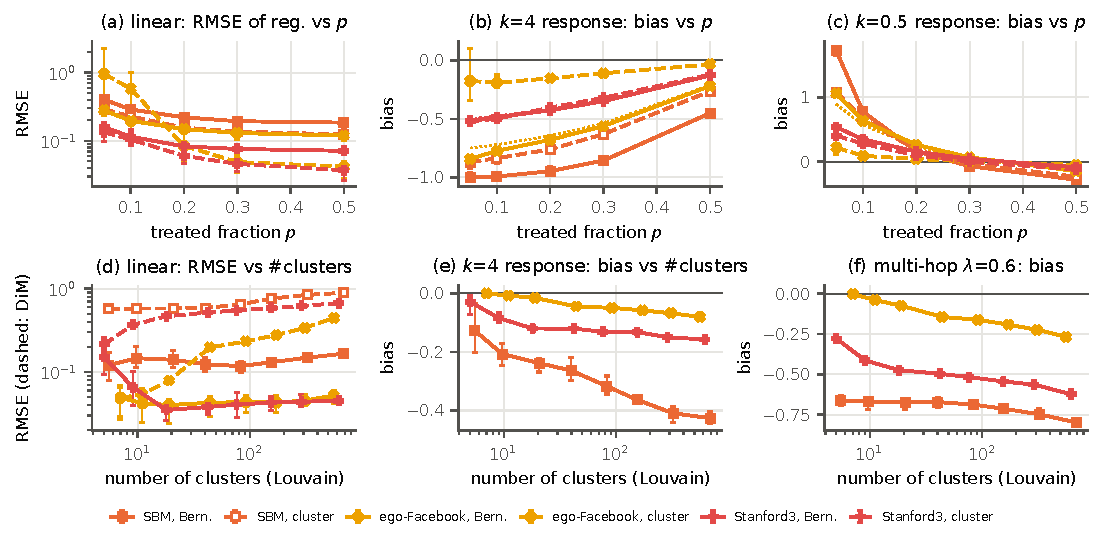
\includegraphics[width=\linewidth]{figs/fig_design.pdf}
\caption{Design factors (E5), \textsc{ols-s} estimator. Top: treated fraction $p$ (solid Bernoulli; dashed cluster randomization with $\approx$30/40 clusters; dotted: closed-form bias for Bernoulli). Bottom: number of clusters (same colours/markers per graph; solid: \textsc{ols-s}, dashed in (d): DiM). Mean over 6 worlds, bars min--max.}
\label{fig:des}
\end{figure}

\subsection{When is regression better than the baselines? (H6)}
\textbf{Difference in means.} In the linear one-hop model DiM estimates only the direct effect, so its bias is $-\bar\gamma$ ($-1.00$ at $\gamma=1$ under Bernoulli on every graph), independent of $n$, whereas the regression is unbiased but pays leverage $L\ge1/v$. The regression has lower RMSE than DiM only when the spillover exceeds roughly the regression's own noise floor, $\gamma^\ast\approx\hat\kappa\sqrt{L/n}$ (Fig.~\ref{fig:cross}). Across nine (degree, $n$) combinations on ER graphs, the measured crossover (RMSE ratio $=1$, log-interpolated, mean of 6 worlds) is within $0.67$--$1.02\times$ of $\hat\kappa\sqrt{L/n}$ (Table~\ref{tab:cross}). It is large for dense graphs and small samples: with $n=10^3$, $d=128$ the spillover must be $0.82\beta$ before regression helps, whereas at $n=1.6\times10^4$, $d=8$ it is $0.03\beta$. When there is no interference ($\gamma=0$) DiM is better by a factor $\sqrt{L v}=\sqrt{1+d_H}$ (RMSE $0.016$ vs $0.047$ at $d=8$, $n=1.6\times10^4$; $0.032$ vs $0.38$ at $d=128$, $n=4000$). On the real graphs the crossover is at $\gamma\approx0.07$ (Stanford3) and $\approx0.12$ (ego-Facebook) under Bernoulli design and at $\approx0.06$ and $\approx0.19$ under cluster randomization (Fig.~\ref{fig:cross}c; read off the grid $\gamma\in\{0,0.05,0.1,0.2,\dots\}$ by interpolation).

\textbf{H\'ajek.} The full-neighbourhood H\'ajek estimator is unbiased when defined but is undefined in $79\%$ of draws at $d=16$ ($n=4000$) and $100\%$ for $d\ge32$ under Bernoulli (Appendix Table~\ref{tab:cross}); where defined its RMSE is $1.3$--$1.6$ on ER. On Stanford3 and ego-Facebook, whose low-degree units supply qualifying exposures, it is defined and unbiased but has RMSE $0.48$ and $0.67$ under Bernoulli versus $0.07$ and $0.12$ for the regression; with $\approx30$ clusters it is competitive on ego-Facebook ($0.070$ vs $0.042$) and worse on Stanford3 ($0.179$ vs $0.037$). With strongly nonlinear responses and cluster randomization on ego-Facebook it matches the linear regression (threshold: $0.07$ vs $0.07$; $k{=}4$: $0.07$ vs $0.08$), so on clusterable graphs it is a safe alternative.

\begin{figure}[t]
\centering
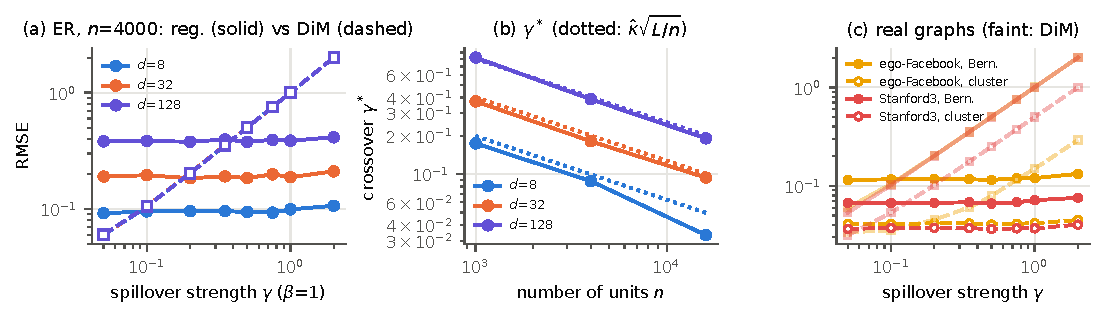
\includegraphics[width=\linewidth]{figs/fig_crossover.pdf}
\caption{Regression vs DiM (E4). (a) RMSE vs $\gamma$ on ER graphs ($n{=}4000$, $\beta{\approx}1$): regression (solid) is flat at its noise floor, DiM (dashed) grows with its bias. (b) Spillover strength at which both have equal RMSE vs $n$ for three degrees; dotted: $\hat\kappa\sqrt{L/n}$. (c) Real graphs, Bernoulli (solid) and clustered (dashed; hollow), regression in colour, DiM faint. Mean over 6 worlds.}
\label{fig:cross}
\end{figure}

\subsection{Confidence intervals}
We audit three standard errors for the one-hop regression (E6; $R=400\times6$ worlds; 8 graph/design combinations): the HC1 sandwich over units; a sandwich clustered on Louvain communities; and a graph-HAC allowing residuals of units within two hops to correlate~\citep{kojevnikov2021limit} (coverage in Appendix Fig.~\ref{fig:inf}). \emph{Correct model:} HC coverage is near nominal (mean $0.95$, range $0.87$--$1.00$ over the 48 world-settings; mean SE/SD ratio $1.03$); the clustered sandwich is slightly anticonservative ($0.93$, ratio $0.97$) and the HAC more so ($0.88$, ratio $0.91$; $0.79$ for ER with $d=30$), its 2-hop pattern covering $4\%$--$34\%$ of all pairs. \emph{Misspecified models} (concave $k=\frac12$, multi-hop $\lambda=0.4$): HC coverage has mean $0.57$ (range $0.06$--$0.83$; lowest on Stanford3 where the bias is $3.2$ SD). This is a bias problem: coverage predicted from the observed bias, SD and mean SE under a normal approximation matches the observed one with mean absolute difference $0.011$ (correlation $0.998$, 144 world-settings). The exception is clustered designs with misspecification, where the HC SE underestimates the SD (ratio $0.46$ for Stanford3/concave, $0.58$ for ego-Facebook/multi-hop; clustered sandwich $0.79$, $0.89$). No variance estimator addresses $B$: intervals cover the regression's population target, not the GATE.



\subsection{A mis-measured network}
The interference graph is itself an estimate. In E7 exposure features are computed from a graph in which a fraction $f$ of true edges is replaced by random edges (outcomes follow the true graph, linear response). Under Bernoulli designs the one-hop regression is attenuated towards the direct effect by almost exactly $f\bar\gamma$ (App.\ Fig.~\ref{fig:obs}a): bias $-0.06,-0.11,-0.22,-0.42$ for $f=0.05,0.1,0.2,0.4$ on Stanford3 (ego-Facebook, ER alike), RMSE $0.07\to0.45$. Under cluster randomization the degradation is milder in our runs (Stanford3: bias $-0.03$, RMSE $0.037\to0.087$ at $f=0.4$; ego-Facebook: bias $+0.07$, RMSE $0.042\to0.118$); we did not investigate why, and clusters were computed on the true graph, which flatters this case. The two-step model is more fragile (bias $+0.23$ at $f=0.05$ on Stanford3, Bernoulli).



\section{Discussion and limitations}
\label{sec:disc}

\textbf{What determines the error.} In our experiments the RMSE of the regression GATE estimator is well described by $\sqrt{B^2+\hat\kappa^2L/n}$ (Fig.~\ref{fig:ext}d). $L$ depends only on graph and design and can be computed \emph{before} an experiment (Prop.~\ref{prop:lev}): it grows with the harmonic-mean degree and $1/(p(1-p))$ and is cut by clusterings that keep neighbourhoods together. $B$ is what the regression cannot represent: the response slope away from the exposures the design visits, interference beyond the modelled neighbourhood, and effect heterogeneity correlated with a unit's exposure variance. More data does not cure a nonzero $B$; a larger model helps only where the design or low-degree units provide support, and otherwise trades bias for leverage. Practically: (i) use $L$ to size experiments and pick $p$ (near $\frac12$) and the clustering; (ii) prefer cluster randomization when the graph is clusterable, balancing bias against the number of independent units; (iii) comparing with richer specifications is a natural sensitivity check, but their leverage was up to $20\times$ larger, so only large biases are detectable (not evaluated formally); (iv) intervals inherit $B$.

\textbf{Limitations.} \emph{Synthetic outcomes:} four stylized mechanisms with chosen parameters ($\gamma{=}1$, $\lambda\le0.8$); bias magnitudes belong to these, not to platforms, and real interference may combine them or add attribute heterogeneity and dynamics. \emph{Known graph} except in E7 (one of many mis-measurement models). \emph{Theory:} Props.~\ref{prop:decomp}--\ref{prop:mh} are first-order design-expectation statements without rates; there is no closed form for $B$ under cluster designs, and the leverage formula underpredicts RMSE in 73\% of cluster-design runs (median $+10\%$, up to $3.7\times$). \emph{Estimators:} hand-specified exposure features, two heterogeneity fixes and one boosting model (few replications); we did not implement the covariate selection of~\citep{han2023model}, regularized fits or optimized clusterings (Louvain, unequal sizes). \emph{Inference:} three variance estimators, none correcting bias. \emph{Scale:} $\le1.2\times10^4$ nodes, 6 worlds per setting, bars are min--max not confidence intervals. \emph{Pilot:} \textsc{wls-s}/\textsc{strat-s} were designed after the heterogeneity pilot, so Table~\ref{tab:het} is in-sample for them. Negative results (little clustering benefit on weakly clusterable graphs, no help from quadratic terms, two-step exposure raising RMSE, anticonservative HAC, biased boosting) are reported in Sec.~\ref{sec:results}.


\bibliographystyle{plainnat}
\bibliography{refs}

\appendix
\section{Proofs}
\label{app:proofs}

\paragraph{Pooled moments.} Because the design is symmetric across units and we average over units, all moments below are \emph{pooled}: $\Sigma=\frac1n\sum_i\mathbb E[\phi_i\phi_i^\top]$. If $\phi$ contains an intercept and $\bar d$ has a zero intercept coordinate, then $\bar d^\top\Sigma^{-1}\bar d=\tilde d^\top\Gamma^{-1}\tilde d$, where $\Gamma$ is the pooled covariance matrix of the non-intercept features and $\tilde d$ the corresponding sub-vector of $\bar d$ (block inverse / Schur complement).

\begin{proof}[Proof of Proposition~\ref{prop:decomp}]
$\hat\beta=\hat\Sigma^{-1}\frac1n\sum_i\phi_i(\phi_i^\top\beta^\star+\varepsilon_i)=\beta^\star+\hat\Sigma^{-1}\hat g$, so $\hat\tau-\tau=(\bar d^\top\beta^\star-\tau)+\bar d^\top\hat\Sigma^{-1}\hat g$. By definition of $\beta^\star$, $\mathbb E\hat g=\frac1n\sum_i\mathbb E[\phi_iy_i]-\Sigma\beta^\star=0$. Replacing $\hat\Sigma$ by $\Sigma$ the second term is $u^\top\Sigma^{-1/2}\hat g$ with $u=\Sigma^{-1/2}\bar d$, $\|u\|^2=L$; its variance is $u^\top M u/n$ with $M=\Sigma^{-1/2}\,n\mathrm{Cov}(\hat g)\,\Sigma^{-1/2}$, and $u^\top Mu\le\lambda_{\max}(M)\|u\|^2=\kappa L$ (Rayleigh quotient). The replacement of $\hat\Sigma$ by $\Sigma$ is a first-order (delta-method) approximation; we do not prove a rate and instead test its consequence ($\mathrm{RMSE}\approx\sqrt{B^2+\kappa L/n}$) empirically.
\end{proof}

\begin{proof}[Proof of Proposition~\ref{prop:lev}]
Take $\phi=(1,z,s)$, $\bar d=(0,1,1)$. Since $s_i=\sum_jW_{ij}z_j$ and $\mathbb E z_j=p$, $\mathbb E s_i=p$. Under independent cluster-level Bernoulli assignment $\mathrm{Cov}(z_j,z_l)=v\,\mathbf 1[c(j)=c(l)]$. Hence $\Gamma_{zz}=v$; $\mathrm{Cov}(z_i,s_i)=v\sum_jW_{ij}\mathbf 1[c(j)=c(i)]=v\,w_{i,c(i)}$, so $\Gamma_{zs}=v\rho$; and $\mathrm{Var}(s_i)=v\sum_c(m_{ic}/d_i)^2$, so $\Gamma_{ss}=vq$. With $\tilde d=(1,1)$,
$\tilde d^\top\Gamma^{-1}\tilde d=\frac1v\frac{1-2\rho+q}{q-\rho^2}=\frac1v\big[1+\frac{(1-\rho)^2}{q-\rho^2}\big]$. $q\ge\rho^2$ by Jensen and $\sum_cw_{ic}^2\ge w_{i,c(i)}^2$. For unit randomization $m_{ic}\in\{0,1\}$ for singleton clusters, $\rho=0$, $q=\frac1n\sum_i 1/d_i=1/d_H$.
\end{proof}

\begin{proof}[Proof of Proposition~\ref{prop:extrap}]
Under Bernoulli assignment $s_i=\frac1{d_i}\sum_{j\sim i}z_j$ is independent of $z_i$ (no self loops), $\mathbb E s_i=p$, $s_i\sim\mathrm{Bin}(d_i,p)/d_i$ and $\mathrm{Var}(s_i)=v/d_i$. Thus $\Gamma_{zs}=0$, $\Gamma_{zz}=v$, $\Gamma_{ss}=\frac1n\sum_iv/d_i$. The fixed baselines $a_i$ have zero pooled covariance with $z$ and $s$ because $\mathbb E z_i=\mathbb E s_i=p$ for all $i$. Therefore the pooled covariances of $y$ with $z$ and $s$ are $v\bar\beta$ and $\gamma\frac1n\sum_i\mathrm{Cov}(g(s_i),s_i)$ (the term $\beta_i\mathrm{Cov}(z_i,s_i)$ vanishes and $\mathrm{Cov}(g(s_i),z_i)=0$), giving the coefficients $\bar\beta$ and $\gamma\kappa_p$ on $z$ and $s$; $\bar d^\top\beta^\star=\bar\beta+\gamma\kappa_p$ while $\tau=\bar\beta+\gamma(g(1)-g(0))$. For the limit, $s_i-p=O_P(d_i^{-1/2})$; for $g\in C^2$, $\mathrm{Cov}(g(s),s)=g'(p)\mathrm{Var}(s)+O(\mathbb E|s-p|^3)=g'(p)\mathrm{Var}(s)+O(d^{-3/2})$ hence $\kappa_p\to g'(p)$ as $\min_id_i\to\infty$. (For $g(s)=s^2$ and $p=\frac12$ one finds $\kappa_p=1$ exactly for every $d$.) The quantity $\kappa_p$ is evaluated by exact binomial sums for each observed degree in our code (\texttt{theory.py}).
\end{proof}

\begin{proof}[Proof of Proposition~\ref{prop:wt}]
As above $\Gamma_{zz}=v$, $\Gamma_{zs}=0$, $\Gamma_{ss}=v\,\frac1n\sum_id_i^{-1}$. Pooled $\mathrm{Cov}(y,z)=v\bar\beta$ and $\mathrm{Cov}(y,s)=\frac1n\sum_i\gamma_i\mathrm{Var}(s_i)=\frac vn\sum_i\gamma_id_i^{-1}$. The coefficient on $s$ is $\sum_i\gamma_id_i^{-1}/\sum_jd_j^{-1}=\sum_i\pi_i\gamma_i$.
\end{proof}

\begin{proof}[Proof of Proposition~\ref{prop:mh}]
$Y(z)=\sum_{k\ge0}\lambda^kW^k(a+\beta z)$ (Neumann series). Under Bernoulli assignment $\mathrm{Cov}(z_i,(W^kz)_i)=v(W^k)_{ii}$ and $\mathrm{Cov}(s_i,(W^kz)_i)=v\sum_jW_{ij}(W^k)_{ij}$. Pooling over $i$ and using $\Gamma_{zs}=0$, $\Gamma_{zz}=v$, $\Gamma_{ss}=vq$: the coefficient on $z$ is $\beta\sum_{k\ge0}\lambda^kr_k=\beta(1+\sum_{k\ge2}\lambda^kr_k)$ ($r_0=1$, $r_1=0$) and the coefficient on $s$ is $\beta\sum_{k\ge1}\lambda^ku_k/q=\beta(\lambda+\sum_{k\ge2}\lambda^ku_k/q)$. Their sum minus $\tau=\beta\sum_{k\ge0}\lambda^k$ is $-\beta\sum_{k\ge2}\lambda^k(1-\psi_k)$. On locally tree-like, high-degree graphs $r_k,u_k/q\to0$ for $k\ge2$ and $B\to-\beta\lambda^2/(1-\lambda)$.
\end{proof}

\section{Additional results}
\label{app:extra}
\begin{table}[h]\centering\footnotesize
\caption{Closed-form leverage vs simulation (E1, \textsc{ols-s}). Runs are (setting, world) pairs. Left: simulated mean leverage over $R$ assignments divided by $L$ of Prop.~\ref{prop:lev}; right: observed RMSE divided by $\hat\kappa\sqrt{L/n}$ (median [min, max]).}
\label{tab:lev}\begin{tabular}{lrcc}\toprule
family/design & runs & $\bar L_{\rm sim}/L$ & RMSE / predicted \\
\midrule
BA/Bern. & 24 & 1.01 [1.00, 1.02] & 1.01 [0.91, 1.05] \\
BA/cluster & 24 & 1.40 [1.10, 2.33] & 1.23 [0.90, 1.66] \\
ER/Bern. & 72 & 1.01 [1.00, 1.07] & 1.01 [0.89, 1.10] \\
SBM/Bern. & 30 & 1.01 [1.00, 1.04] & 1.00 [0.92, 1.10] \\
SBM/cluster & 30 & 1.36 [1.12, 2.65] & 1.20 [0.85, 1.75] \\
Stanford3/Bern. & 6 & 1.00 [1.00, 1.00] & 1.03 [0.98, 1.09] \\
Stanford3/cluster & 24 & 1.15 [1.05, 15.57] & 1.11 [0.77, 3.74] \\
WS/Bern. & 24 & 1.01 [1.00, 1.03] & 1.00 [0.91, 1.08] \\
WS/cluster & 24 & 1.03 [1.03, 1.04] & 1.00 [0.85, 1.19] \\
ego-Facebook/Bern. & 6 & 1.02 [1.02, 1.02] & 1.05 [0.85, 1.13] \\
ego-Facebook/cluster & 24 & 1.07 [1.03, 1.30] & 1.08 [0.69, 1.50] \\
\bottomrule\end{tabular}\end{table}

\begin{table}[h]\centering\footnotesize
\caption{Dependence on the baseline scale $\sigma_a$ (E1; ER, $n=4000$, $d=16$, Bernoulli; effect heterogeneity fixed at $0.5$).}
\label{tab:siga}\begin{tabular}{rrr}\toprule
$\sigma_a$ & RMSE & bias \\
\midrule
0.25 & 0.065 & -0.002 \\
0.50 & 0.085 & +0.004 \\
1.00 & 0.132 & +0.003 \\
2.00 & 0.254 & -0.004 \\
4.00 & 0.503 & -0.002 \\
\bottomrule\end{tabular}\end{table}

\begin{table}[h]\centering\footnotesize
\caption{Clustering quality and error (E5, linear response, \textsc{ols-s}, $p=\frac12$): number of Louvain clusters, fraction of edges cut, simulated mean leverage, closed-form leverage, RMSE (means over 6 worlds).}
\label{tab:clu}\begin{tabular}{lrrrrr}\toprule
graph & clusters & cut & $\bar L_{\rm sim}$ & $L$ & RMSE \\
\midrule
SBM & 6 & 0.44 & 72.3 & 13.7 & 0.120 \\
SBM & 10 & 0.50 & 61.6 & 21.5 & 0.146 \\
SBM & 21 & 0.55 & 55.5 & 31.7 & 0.140 \\
SBM & 40 & 0.57 & 54.4 & 40.5 & 0.124 \\
SBM & 83 & 0.63 & 43.5 & 35.9 & 0.117 \\
SBM & 154 & 0.75 & 51.8 & 45.7 & 0.131 \\
SBM & 324 & 0.84 & 72.5 & 67.3 & 0.148 \\
SBM & 690 & 0.89 & 91.1 & 87.5 & 0.166 \\
Stanford3 & 5 & 0.02 & 461.3 & 4.3 & 0.151 \\
Stanford3 & 9 & 0.34 & 56.2 & 7.3 & 0.066 \\
Stanford3 & 18 & 0.53 & 14.1 & 10.4 & 0.035 \\
Stanford3 & 42 & 0.61 & 14.8 & 12.6 & 0.038 \\
Stanford3 & 76 & 0.67 & 15.4 & 13.9 & 0.040 \\
Stanford3 & 155 & 0.72 & 16.5 & 15.4 & 0.043 \\
Stanford3 & 288 & 0.76 & 17.6 & 16.7 & 0.044 \\
Stanford3 & 621 & 0.81 & 20.4 & 19.8 & 0.045 \\
ego-Facebook & 7 & 0.00 & 6.6 & 4.1 & 0.049 \\
ego-Facebook & 11 & 0.03 & 5.5 & 4.3 & 0.042 \\
ego-Facebook & 19 & 0.06 & 5.3 & 4.6 & 0.040 \\
ego-Facebook & 44 & 0.32 & 5.9 & 5.5 & 0.043 \\
ego-Facebook & 92 & 0.41 & 6.2 & 5.8 & 0.043 \\
ego-Facebook & 172 & 0.49 & 6.7 & 6.4 & 0.043 \\
ego-Facebook & 310 & 0.58 & 7.4 & 7.1 & 0.045 \\
ego-Facebook & 559 & 0.70 & 9.0 & 8.7 & 0.052 \\
\bottomrule\end{tabular}\end{table}

\begin{table}[t]\centering\footnotesize
\caption{Crossover spillover strength $\gamma^\ast$ above which the one-hop regression has lower RMSE than DiM (E4; ER graphs, Bernoulli; $\beta\approx1$), versus $\hat\kappa\sqrt{L/n}$; RMSE of DiM and regression at $\gamma=0$. H\'ajek (E1, $n=4000$) is undefined in a fraction 0.00, 0.00, 0.79, 1.00, 1.00, 1.00, 1.00 of draws for $d=4,8,16,32,64,128,256$ respectively.}
\label{tab:cross}\begin{tabular}{rrrrrr}\toprule
$d$ & $n$ & $\gamma^\ast$ (obs.) & $\hat\kappa\sqrt{L/n}$ & DiM RMSE & reg. RMSE \\
\midrule
8 & 1000 & 0.174 & 0.199 & 0.064 & 0.190 \\
8 & 4000 & 0.088 & 0.099 & 0.033 & 0.095 \\
8 & 16000 & 0.033 & 0.050 & 0.016 & 0.047 \\
32 & 1000 & 0.372 & 0.402 & 0.064 & 0.376 \\
32 & 4000 & 0.181 & 0.201 & 0.032 & 0.191 \\
32 & 16000 & 0.094 & 0.100 & 0.017 & 0.094 \\
128 & 1000 & 0.823 & 0.805 & 0.067 & 0.822 \\
128 & 4000 & 0.387 & 0.402 & 0.032 & 0.380 \\
128 & 16000 & 0.191 & 0.201 & 0.016 & 0.187 \\
\bottomrule\end{tabular}\end{table}


\paragraph{Notes.} (i) In Table~\ref{tab:lev} the closed-form leverage is essentially exact for Bernoulli designs (within $7\%$ in every run, within $2\%$ in the median family) and underestimates the simulated leverage for cluster designs, by a median of $3$--$40\%$ per family and by a factor up to $15.6$ (Stanford3 with 9 clusters), consistent with Prop.~\ref{prop:lev} being an expectation over assignments. (ii) In Table~\ref{tab:clu} the closed-form leverage is accurate once there are about $\ge20$ clusters. (iii) Table~\ref{tab:siga}: RMSE scales sublinearly in $\sigma_a$ because effect heterogeneity (coefficients $\beta_i,\gamma_i$ with 50\% relative SD) adds a baseline-independent component.

\begin{table}[t]\centering\footnotesize\setlength{\tabcolsep}{3.5pt}
\caption{Nonlinear exposure response (E2): bias (RMSE) of the GATE estimate; true GATE $\approx2$. Mean over 6 worlds ($R{=}300$). $^\dagger$ \textsc{gbm}: 3 worlds, $R{=}40$ assignments each. ``--'': H\'ajek undefined in $\ge50\%$ of draws (or not run).}
\label{tab:extrap}
\begin{tabular}{lllccccc}\toprule
graph & response & design & \textsc{ols-s} & +$s^2$ & +$s^2,s^3$ & \textsc{gbm}$^\dagger$ & H\'ajek \\
\midrule
ER & k=4 & Bern. & -0.45 (0.50) & -0.45 (0.50) & +0.01 (1.92) & -0.65 (0.83) & -- \\
 &  & cluster & -0.36 (0.52) & -0.45 (0.54) & +0.03 (1.51) & -0.60 (0.72) & -- \\
 & threshold & Bern. & +1.46 (1.48) & +1.47 (1.49) & -2.34 (3.06) & -0.14 (0.52) & -- \\
 &  & cluster & +0.94 (1.02) & +1.48 (1.52) & -0.65 (2.27) & -0.08 (0.41) & -- \\
ego-Facebook & k=4 & Bern. & -0.22 (0.30) & -0.24 (0.27) & -0.01 (0.17) & -0.17 (0.49) & -0.01 (0.65) \\
 &  & cluster & -0.03 (0.08) & -0.03 (0.06) & +0.00 (0.05) & -0.01 (0.22) & -0.00 (0.07) \\
 & threshold & Bern. & +0.60 (0.61) & +0.64 (0.66) & -0.07 (0.18) & +0.12 (0.41) & -0.01 (0.63) \\
 &  & cluster & +0.05 (0.07) & +0.05 (0.07) & -0.01 (0.05) & -0.01 (0.25) & -0.00 (0.07) \\
Stanford3 & k=4 & Bern. & -0.13 (0.15) & -0.13 (0.15) & -0.01 (0.08) & -0.26 (0.37) & -0.01 (0.50) \\
 &  & cluster & -0.12 (0.21) & -0.13 (0.14) & -0.00 (0.06) & -0.11 (0.21) & -0.00 (0.17) \\
 & threshold & Bern. & +0.37 (0.37) & +0.37 (0.37) & -0.03 (0.09) & -0.11 (0.26) & -0.03 (0.48) \\
 &  & cluster & +0.20 (0.20) & +0.23 (0.24) & -0.06 (0.08) & -0.06 (0.14) & +0.00 (0.16) \\
\bottomrule\end{tabular}\end{table}

\begin{table}[t]\centering\footnotesize\setlength{\tabcolsep}{3.5pt}
\caption{Multi-hop spillover, $\lambda=0.6$ (E3): bias (RMSE) of DiM, one-hop regression and regression with two-step exposure; last two columns: closed-form bias of the one-hop regression under Bernoulli designs (exact walk-statistics formula, tree-like approximation). Mean over 6 worlds.}
\label{tab:mh}
\begin{tabular}{llccccc}\toprule
graph/design & GATE & DiM & \textsc{ols-s} & \textsc{ols-s2} & $B$ exact & $B$ tree \\
\midrule
ER/Bern. & 2.49 & -1.48 (1.48) & -0.87 (0.89) & -0.55 (1.19) & -0.867 & -0.900 \\
SBM/Bern. & 2.49 & -1.49 (1.49) & -0.86 (0.88) & -0.48 (1.16) & -- & -0.900 \\
SBM/cluster & 2.49 & -1.15 (1.15) & -0.67 (0.69) & -0.43 (0.83) & -- & -- \\
ego-FB/Bern. & 2.49 & -1.47 (1.47) & -0.71 (0.76) & -0.22 (0.65) & -0.696 & -0.900 \\
ego-FB/cluster & 2.49 & -0.34 (0.35) & -0.11 (0.16) & -0.02 (0.13) & -- & -- \\
Stanford3/Bern. & 2.50 & -1.49 (1.49) & -0.85 (0.85) & -0.42 (0.55) & -0.850 & -0.900 \\
Stanford3/cluster & 2.50 & -1.01 (1.01) & -0.49 (0.50) & -0.20 (0.23) & -- & -- \\
\bottomrule\end{tabular}\end{table}


\begin{figure}[h]
\centering
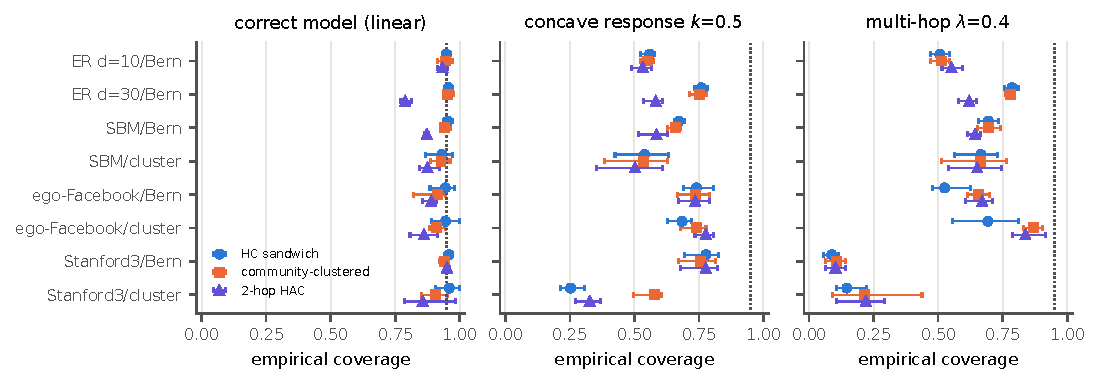
\includegraphics[width=\linewidth]{figs/fig_inference.pdf}
\caption{Coverage of nominal 95\% intervals for the one-hop regression estimator (E6). Markers: mean over 6 worlds; bars min--max. Dotted: 0.95.}
\label{fig:inf}
\end{figure}

\begin{figure}[h]
\centering
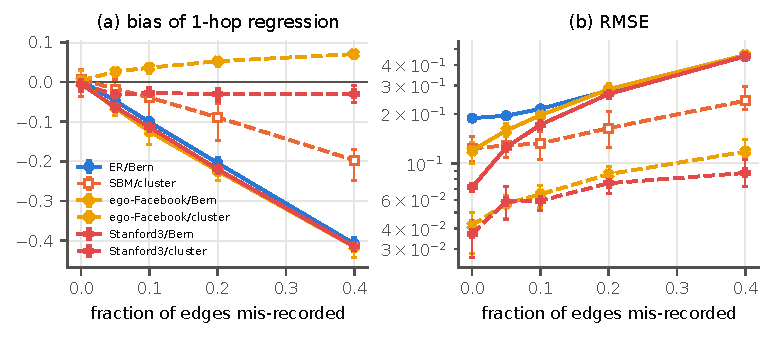
\includegraphics[width=0.62\linewidth]{figs/fig_obsnoise.pdf}
\caption{Mis-measured network (E7): (a) bias and (b) RMSE of the one-hop regression vs fraction of edges replaced by random edges (mean over 6 worlds; bars min--max).}
\label{fig:obs}
\end{figure}


\section{Reproducibility details}
\label{app:repro}
\textbf{Code and instructions.} All code, raw results (CSV), logs and this paper's source are in the released archive; \texttt{README.md} gives the full procedure and \texttt{run\_all\_experiments.sh} runs it end to end. \textbf{Environment:} Python 3.11.2; numpy 2.4.6, scipy 1.17.1, networkx 3.6.1, pandas 3.1.1, scikit-learn 1.9.1, matplotlib 3.11.2 (\texttt{requirements.txt}); pdfLaTeX (TeX Live) with the official \texttt{neurips\_2026.sty}. \textbf{Hardware/time:} CPU only; the container was limited to 4 CPU cores (cgroup quota) with 251\,GB RAM available (memory use was not profiled; each worker held at most one graph and, for E6's HAC, one $\approx10^7$--$10^8$-entry sparse matrix). Wall-clock times of the final runs on 4 processes: E1 172\,s, E2 473\,s, E2g (boosting) 181\,s, E3 355\,s, E4 177\,s, E5 1269\,s, E6 858\,s, E7 64\,s, exact walk statistics (\texttt{psi.py}) $\approx4$\,min; about $1$\,h in total ($\approx4$ CPU-hours); the 3-world pilot of E1/E3 cost a few minutes.
\textbf{Data.} Stanford3: \url{https://nrvis.com/download/data/socfb/socfb-Stanford3.zip} (Network Repository, CC BY-SA; original source Traud et al.~\citep{traud2012social}; file \texttt{socfb-Stanford3.mtx}, $11586\times11586$, 568{,}309 edges; zip SHA-256 \texttt{b1221e41\ldots e8720d}, verified, 1{,}649{,}740 bytes). ego-Facebook: \url{https://snap.stanford.edu/data/facebook_combined.txt.gz} (SNAP; McAuley and Leskovec~\citep{mcauley2012learning}; 88{,}234 edges, 4{,}039 nodes; SHA-256 \texttt{125e84db\ldots 35d7}, verified, 218{,}576 bytes). Downloads are parsed as plain text only (never executed) by \texttt{code/graphs.py}; both graphs are connected so the largest-component restriction is the identity. Synthetic graphs use \texttt{networkx}.
\textbf{Seeds.} Synthetic graph of world $i$: seed $100+i$; outcome parameters of world $i$: seed $1000+i$ ($i=0..5$); the assignment RNG of each configuration is seeded by the first 8 hex digits of the SHA-256 of its (graph, mechanism, design, $i$) description (\texttt{experiments.stable\_seed}); Louvain clustering uses seed 1 (cached on disk for the real graphs). We re-ran E7 and obtained bit-identical numeric output (the other experiments use the same mechanism; they were not re-run end to end).
\textbf{Script $\to$ output.} Fig.~1 \texttt{fig\_variance.py} (E1); Fig.~2 \texttt{fig\_extrap.py} (E2; $\hat\kappa$ from \texttt{stats\_summary.py}); Fig.~3 \texttt{fig\_multihop.py} (E3, \texttt{psi.py}); Fig.~4 \texttt{fig\_crossover.py} (E4); Fig.~5 \texttt{fig\_design.py} (E5); Figs.~6--7 \texttt{fig\_inference.py}, \texttt{fig\_obsnoise.py} (E6, E7); Table~1 \texttt{mk\_tables.py:tab\_het} (E3); Tables~2--7 \texttt{mk\_tables.py} (E1--E5); every number quoted in the text is printed by \texttt{stats\_summary.py} or \texttt{verify\_claims.py}. \textbf{Literature access.} Only the starter literature and unrelated public papers were consulted (searches by title for the cited works). No page matching the withheld paper was knowingly opened; a few search-result titles/abstract snippets of unrelated network-interference papers were seen incidentally and none was read further.


\newpage
\section*{NeurIPS Paper Checklist}




\begin{enumerate}

\item {\bf Claims}
    \item[] Question: Do the main claims made in the abstract and introduction accurately reflect the paper's contributions and scope?
    \item[] Answer: \answerYes{}
    \item[] Justification: The abstract and introduction state the findings (closed-form leverage/bias predictors, their validation, baselines, coverage) and the scope (synthetic outcomes, two Facebook graphs); Sec.~\ref{sec:intro}, \ref{sec:results}, \ref{sec:disc}.
    \item[] Guidelines:
    \begin{itemize}
        \item The answer \answerNA{} means that the abstract and introduction do not include the claims made in the paper.
        \item The abstract and/or introduction should clearly state the claims made, including the contributions made in the paper and important assumptions and limitations. A \answerNo{} or \answerNA{} answer to this question will not be perceived well by the reviewers. 
        \item The claims made should match theoretical and experimental results, and reflect how much the results can be expected to generalize to other settings. 
        \item It is fine to include aspirational goals as motivation as long as it is clear that these goals are not attained by the paper. 
    \end{itemize}

\item {\bf Limitations}
    \item[] Question: Does the paper discuss the limitations of the work performed by the authors?
    \item[] Answer: \answerYes{}
    \item[] Justification: Sec.~\ref{sec:disc} (Limitations) lists synthetic outcomes, known graph, first-order theory, approximate cluster-design formula, limited estimator family and inference, 6 worlds, and the post-pilot design of two estimators.
    \item[] Guidelines:
    \begin{itemize}
        \item The answer \answerNA{} means that the paper has no limitation while the answer \answerNo{} means that the paper has limitations, but those are not discussed in the paper. 
        \item The authors are encouraged to create a separate ``Limitations'' section in their paper.
        \item The paper should point out any strong assumptions and how robust the results are to violations of these assumptions (e.g., independence assumptions, noiseless settings, model well-specification, asymptotic approximations only holding locally). The authors should reflect on how these assumptions might be violated in practice and what the implications would be.
        \item The authors should reflect on the scope of the claims made, e.g., if the approach was only tested on a few datasets or with a few runs. In general, empirical results often depend on implicit assumptions, which should be articulated.
        \item The authors should reflect on the factors that influence the performance of the approach. For example, a facial recognition algorithm may perform poorly when image resolution is low or images are taken in low lighting. Or a speech-to-text system might not be used reliably to provide closed captions for online lectures because it fails to handle technical jargon.
        \item The authors should discuss the computational efficiency of the proposed algorithms and how they scale with dataset size.
        \item If applicable, the authors should discuss possible limitations of their approach to address problems of privacy and fairness.
        \item While the authors might fear that complete honesty about limitations might be used by reviewers as grounds for rejection, a worse outcome might be that reviewers discover limitations that aren't acknowledged in the paper. The authors should use their best judgment and recognize that individual actions in favor of transparency play an important role in developing norms that preserve the integrity of the community. Reviewers will be specifically instructed to not penalize honesty concerning limitations.
    \end{itemize}

\item {\bf Theory assumptions and proofs}
    \item[] Question: For each theoretical result, does the paper provide the full set of assumptions and a complete (and correct) proof?
    \item[] Answer: \answerYes{}
    \item[] Justification: Props.~\ref{prop:decomp}--\ref{prop:mh} state assumptions; proofs are in Appendix~\ref{app:proofs}. They are design-expectation/first-order statements and are labelled as such (no rates are claimed).
    \item[] Guidelines:
    \begin{itemize}
        \item The answer \answerNA{} means that the paper does not include theoretical results. 
        \item All the theorems, formulas, and proofs in the paper should be numbered and cross-referenced.
        \item All assumptions should be clearly stated or referenced in the statement of any theorems.
        \item The proofs can either appear in the main paper or the supplemental material, but if they appear in the supplemental material, the authors are encouraged to provide a short proof sketch to provide intuition. 
        \item Inversely, any informal proof provided in the core of the paper should be complemented by formal proofs provided in appendix or supplemental material.
        \item Theorems and Lemmas that the proof relies upon should be properly referenced. 
    \end{itemize}

    \item {\bf Experimental result reproducibility}
    \item[] Question: Does the paper fully disclose all the information needed to reproduce the main experimental results of the paper to the extent that it affects the main claims and/or conclusions of the paper (regardless of whether the code and data are provided or not)?
    \item[] Answer: \answerYes{}
    \item[] Justification: Sec.~\ref{sec:setting}, \ref{sec:protocol} and Appendix~\ref{app:repro} give graphs, outcome mechanisms and parameters, designs, estimators, metrics, seeds and versions; every experiment is in the released code.
    \item[] Guidelines:
    \begin{itemize}
        \item The answer \answerNA{} means that the paper does not include experiments.
        \item If the paper includes experiments, a \answerNo{} answer to this question will not be perceived well by the reviewers: Making the paper reproducible is important, regardless of whether the code and data are provided or not.
        \item If the contribution is a dataset and\slash or model, the authors should describe the steps taken to make their results reproducible or verifiable. 
        \item Depending on the contribution, reproducibility can be accomplished in various ways. For example, if the contribution is a novel architecture, describing the architecture fully might suffice, or if the contribution is a specific model and empirical evaluation, it may be necessary to either make it possible for others to replicate the model with the same dataset, or provide access to the model. In general. releasing code and data is often one good way to accomplish this, but reproducibility can also be provided via detailed instructions for how to replicate the results, access to a hosted model (e.g., in the case of a large language model), releasing of a model checkpoint, or other means that are appropriate to the research performed.
        \item While NeurIPS does not require releasing code, the conference does require all submissions to provide some reasonable avenue for reproducibility, which may depend on the nature of the contribution. For example
        \begin{enumerate}
            \item If the contribution is primarily a new algorithm, the paper should make it clear how to reproduce that algorithm.
            \item If the contribution is primarily a new model architecture, the paper should describe the architecture clearly and fully.
            \item If the contribution is a new model (e.g., a large language model), then there should either be a way to access this model for reproducing the results or a way to reproduce the model (e.g., with an open-source dataset or instructions for how to construct the dataset).
            \item We recognize that reproducibility may be tricky in some cases, in which case authors are welcome to describe the particular way they provide for reproducibility. In the case of closed-source models, it may be that access to the model is limited in some way (e.g., to registered users), but it should be possible for other researchers to have some path to reproducing or verifying the results.
        \end{enumerate}
    \end{itemize}


\item {\bf Open access to data and code}
    \item[] Question: Does the paper provide open access to the data and code, with sufficient instructions to faithfully reproduce the main experimental results, as described in supplemental material?
    \item[] Answer: \answerYes{}
    \item[] Justification: Code, raw results and a README with commands, versions, seeds and data checksums are provided; both graphs are public (Appendix~\ref{app:repro}).
    \item[] Guidelines:
    \begin{itemize}
        \item The answer \answerNA{} means that paper does not include experiments requiring code.
        \item Please see the NeurIPS code and data submission guidelines (\url{https://neurips.cc/public/guides/CodeSubmissionPolicy}) for more details.
        \item While we encourage the release of code and data, we understand that this might not be possible, so \answerNo{} is an acceptable answer. Papers cannot be rejected simply for not including code, unless this is central to the contribution (e.g., for a new open-source benchmark).
        \item The instructions should contain the exact command and environment needed to run to reproduce the results. See the NeurIPS code and data submission guidelines (\url{https://neurips.cc/public/guides/CodeSubmissionPolicy}) for more details.
        \item The authors should provide instructions on data access and preparation, including how to access the raw data, preprocessed data, intermediate data, and generated data, etc.
        \item The authors should provide scripts to reproduce all experimental results for the new proposed method and baselines. If only a subset of experiments are reproducible, they should state which ones are omitted from the script and why.
        \item At submission time, to preserve anonymity, the authors should release anonymized versions (if applicable).
        \item Providing as much information as possible in supplemental material (appended to the paper) is recommended, but including URLs to data and code is permitted.
    \end{itemize}


\item {\bf Experimental setting/details}
    \item[] Question: Does the paper specify all the training and test details (e.g., data splits, hyperparameters, how they were chosen, type of optimizer) necessary to understand the results?
    \item[] Answer: \answerYes{}
    \item[] Justification: No training in the ML sense; all simulation parameters, numbers of worlds/assignments, clustering procedure and the (few) hyper-parameters of the boosting model are in Sec.~\ref{sec:protocol}, Appendix~\ref{app:repro} and the code.
    \item[] Guidelines:
    \begin{itemize}
        \item The answer \answerNA{} means that the paper does not include experiments.
        \item The experimental setting should be presented in the core of the paper to a level of detail that is necessary to appreciate the results and make sense of them.
        \item The full details can be provided either with the code, in appendix, or as supplemental material.
    \end{itemize}

\item {\bf Experiment statistical significance}
    \item[] Question: Does the paper report error bars suitably and correctly defined or other appropriate information about the statistical significance of the experiments?
    \item[] Answer: \answerYes{}
    \item[] Justification: Results are means over 6 independent worlds with min--max bars; Monte-Carlo error of each RMSE ($R{=}300$) is about $4\%$ and is stated; coverage is reported with across-world ranges. Bars are ranges, not confidence intervals (stated).
    \item[] Guidelines:
    \begin{itemize}
        \item The answer \answerNA{} means that the paper does not include experiments.
        \item The authors should answer \answerYes{} if the results are accompanied by error bars, confidence intervals, or statistical significance tests, at least for the experiments that support the main claims of the paper.
        \item The factors of variability that the error bars are capturing should be clearly stated (for example, train/test split, initialization, random drawing of some parameter, or overall run with given experimental conditions).
        \item The method for calculating the error bars should be explained (closed form formula, call to a library function, bootstrap, etc.)
        \item The assumptions made should be given (e.g., Normally distributed errors).
        \item It should be clear whether the error bar is the standard deviation or the standard error of the mean.
        \item It is OK to report 1-sigma error bars, but one should state it. The authors should preferably report a 2-sigma error bar than state that they have a 96\% CI, if the hypothesis of Normality of errors is not verified.
        \item For asymmetric distributions, the authors should be careful not to show in tables or figures symmetric error bars that would yield results that are out of range (e.g., negative error rates).
        \item If error bars are reported in tables or plots, the authors should explain in the text how they were calculated and reference the corresponding figures or tables in the text.
    \end{itemize}

\item {\bf Experiments compute resources}
    \item[] Question: For each experiment, does the paper provide sufficient information on the computer resources (type of compute workers, memory, time of execution) needed to reproduce the experiments?
    \item[] Answer: \answerYes{}
    \item[] Justification: Appendix~\ref{app:repro}: CPU only, 4-core quota, wall-clock per experiment ($\approx1$ h total, $\approx4$ CPU-hours). Memory was not profiled; this is stated.
    \item[] Guidelines:
    \begin{itemize}
        \item The answer \answerNA{} means that the paper does not include experiments.
        \item The paper should indicate the type of compute workers CPU or GPU, internal cluster, or cloud provider, including relevant memory and storage.
        \item The paper should provide the amount of compute required for each of the individual experimental runs as well as estimate the total compute. 
        \item The paper should disclose whether the full research project required more compute than the experiments reported in the paper (e.g., preliminary or failed experiments that didn't make it into the paper). 
    \end{itemize}
    
\item {\bf Code of ethics}
    \item[] Question: Does the research conducted in the paper conform, in every respect, with the NeurIPS Code of Ethics \url{https://neurips.cc/public/EthicsGuidelines}?
    \item[] Answer: \answerYes{}
    \item[] Justification: The research uses only synthetic outcomes and public graphs; no human subjects or private data.
    \item[] Guidelines:
    \begin{itemize}
        \item The answer \answerNA{} means that the authors have not reviewed the NeurIPS Code of Ethics.
        \item If the authors answer \answerNo, they should explain the special circumstances that require a deviation from the Code of Ethics.
        \item The authors should make sure to preserve anonymity (e.g., if there is a special consideration due to laws or regulations in their jurisdiction).
    \end{itemize}


\item {\bf Broader impacts}
    \item[] Question: Does the paper discuss both potential positive societal impacts and negative societal impacts of the work performed?
    \item[] Answer: \answerNA{}
    \item[] Justification: Methodological/diagnostic study with synthetic outcomes; we see no direct societal impact beyond the general relevance of A/B-testing practice; a limitation is that conclusions may not transfer to real platforms.
    \item[] Guidelines:
    \begin{itemize}
        \item The answer \answerNA{} means that there is no societal impact of the work performed.
        \item If the authors answer \answerNA{} or \answerNo, they should explain why their work has no societal impact or why the paper does not address societal impact.
        \item Examples of negative societal impacts include potential malicious or unintended uses (e.g., disinformation, generating fake profiles, surveillance), fairness considerations (e.g., deployment of technologies that could make decisions that unfairly impact specific groups), privacy considerations, and security considerations.
        \item The conference expects that many papers will be foundational research and not tied to particular applications, let alone deployments. However, if there is a direct path to any negative applications, the authors should point it out. For example, it is legitimate to point out that an improvement in the quality of generative models could be used to generate Deepfakes for disinformation. On the other hand, it is not needed to point out that a generic algorithm for optimizing neural networks could enable people to train models that generate Deepfakes faster.
        \item The authors should consider possible harms that could arise when the technology is being used as intended and functioning correctly, harms that could arise when the technology is being used as intended but gives incorrect results, and harms following from (intentional or unintentional) misuse of the technology.
        \item If there are negative societal impacts, the authors could also discuss possible mitigation strategies (e.g., gated release of models, providing defenses in addition to attacks, mechanisms for monitoring misuse, mechanisms to monitor how a system learns from feedback over time, improving the efficiency and accessibility of ML).
    \end{itemize}
    
\item {\bf Safeguards}
    \item[] Question: Does the paper describe safeguards that have been put in place for responsible release of data or models that have a high risk for misuse (e.g., pre-trained language models, image generators, or scraped datasets)?
    \item[] Answer: \answerNA{}
    \item[] Justification: No model or dataset with misuse risk is released.
    \item[] Guidelines:
    \begin{itemize}
        \item The answer \answerNA{} means that the paper poses no such risks.
        \item Released models that have a high risk for misuse or dual-use should be released with necessary safeguards to allow for controlled use of the model, for example by requiring that users adhere to usage guidelines or restrictions to access the model or implementing safety filters. 
        \item Datasets that have been scraped from the Internet could pose safety risks. The authors should describe how they avoided releasing unsafe images.
        \item We recognize that providing effective safeguards is challenging, and many papers do not require this, but we encourage authors to take this into account and make a best faith effort.
    \end{itemize}

\item {\bf Licenses for existing assets}
    \item[] Question: Are the creators or original owners of assets (e.g., code, data, models), used in the paper, properly credited and are the license and terms of use explicitly mentioned and properly respected?
    \item[] Answer: \answerYes{}
    \item[] Justification: Stanford3 (Network Repository, CC BY-SA; Traud et al., Rossi and Ahmed) and ego-Facebook (SNAP; McAuley and Leskovec) are cited with URLs, versions and checksums in Appendix~\ref{app:repro}; the NeurIPS style file is used unmodified.
    \item[] Guidelines:
    \begin{itemize}
        \item The answer \answerNA{} means that the paper does not use existing assets.
        \item The authors should cite the original paper that produced the code package or dataset.
        \item The authors should state which version of the asset is used and, if possible, include a URL.
        \item The name of the license (e.g., CC-BY 4.0) should be included for each asset.
        \item For scraped data from a particular source (e.g., website), the copyright and terms of service of that source should be provided.
        \item If assets are released, the license, copyright information, and terms of use in the package should be provided. For popular datasets, \url{paperswithcode.com/datasets} has curated licenses for some datasets. Their licensing guide can help determine the license of a dataset.
        \item For existing datasets that are re-packaged, both the original license and the license of the derived asset (if it has changed) should be provided.
        \item If this information is not available online, the authors are encouraged to reach out to the asset's creators.
    \end{itemize}

\item {\bf New assets}
    \item[] Question: Are new assets introduced in the paper well documented and is the documentation provided alongside the assets?
    \item[] Answer: \answerYes{}
    \item[] Justification: The released code and README document the new simulation code, scripts and result files.
    \item[] Guidelines:
    \begin{itemize}
        \item The answer \answerNA{} means that the paper does not release new assets.
        \item Researchers should communicate the details of the dataset\slash code\slash model as part of their submissions via structured templates. This includes details about training, license, limitations, etc. 
        \item The paper should discuss whether and how consent was obtained from people whose asset is used.
        \item At submission time, remember to anonymize your assets (if applicable). You can either create an anonymized URL or include an anonymized zip file.
    \end{itemize}

\item {\bf Crowdsourcing and research with human subjects}
    \item[] Question: For crowdsourcing experiments and research with human subjects, does the paper include the full text of instructions given to participants and screenshots, if applicable, as well as details about compensation (if any)? 
    \item[] Answer: \answerNA{}
    \item[] Justification: No crowdsourcing or human subjects.
    \item[] Guidelines:
    \begin{itemize}
        \item The answer \answerNA{} means that the paper does not involve crowdsourcing nor research with human subjects.
        \item Including this information in the supplemental material is fine, but if the main contribution of the paper involves human subjects, then as much detail as possible should be included in the main paper. 
        \item According to the NeurIPS Code of Ethics, workers involved in data collection, curation, or other labor should be paid at least the minimum wage in the country of the data collector. 
    \end{itemize}

\item {\bf Institutional review board (IRB) approvals or equivalent for research with human subjects}
    \item[] Question: Does the paper describe potential risks incurred by study participants, whether such risks were disclosed to the subjects, and whether Institutional Review Board (IRB) approvals (or an equivalent approval/review based on the requirements of your country or institution) were obtained?
    \item[] Answer: \answerNA{}
    \item[] Justification: No human subjects.
    \item[] Guidelines:
    \begin{itemize}
        \item The answer \answerNA{} means that the paper does not involve crowdsourcing nor research with human subjects.
        \item Depending on the country in which research is conducted, IRB approval (or equivalent) may be required for any human subjects research. If you obtained IRB approval, you should clearly state this in the paper. 
        \item We recognize that the procedures for this may vary significantly between institutions and locations, and we expect authors to adhere to the NeurIPS Code of Ethics and the guidelines for their institution. 
        \item For initial submissions, do not include any information that would break anonymity (if applicable), such as the institution conducting the review.
    \end{itemize}

\item {\bf Declaration of LLM usage}
    \item[] Question: Does the paper describe the usage of LLMs if it is an important, original, or non-standard component of the core methods in this research? Note that if the LLM is used only for writing, editing, or formatting purposes and does \emph{not} impact the core methodology, scientific rigor, or originality of the research, declaration is not required.
    %this research? 
    \item[] Answer: \answerYes{}
    \item[] Justification: The research was carried out by an autonomous AI research agent (an LLM-based coding/writing agent) that designed, coded, ran and wrote up all experiments and the paper; this is a core component of how the work was done and is declared here.
    \item[] Guidelines:
    \begin{itemize}
        \item The answer \answerNA{} means that the core method development in this research does not involve LLMs as any important, original, or non-standard components.
        \item Please refer to our LLM policy in the NeurIPS handbook for what should or should not be described.
    \end{itemize}

\end{enumerate}
\end{document}
